\chapter{Multi-Agent Pipeline Architecture}
\label{chap:prototype_framework}

This chapter introduces the first prototype of the multi-agent fact-checking pipeline. The prototype deliberately uses a simplified 
design -- three fixed domain experts and rule-based aggregation -- to establish a controlled baseline for multi-agent performance and to identify the key limitations that motivate the more advanced framework presented in Chapter~\ref{chap:final_framework}. The 
experiments in this chapter focus on two questions: (i) whether combining multiple expert perspectives improves over single-model 
baselines, and (ii) which aggregation strategy is most effective in this setting.

\section{System Overview}

This section introduces the architecture used in the first multi-agent experiments.
The prototype pipeline follows a simple two-stage design: multiple expert agents assess the same claim in parallel, and an aggregation mechanism combines their outputs into a single binary verdict.
The focus is on controlled comparisons between aggregation strategies (e.g., majority vote, weighted voting, and a decision-agent) while keeping expert prompts and output constraints consistent.

\subsection{Motivation for Multi-Agent Design}

The single-model baselines in the previous chapter showed that factuality classification can be improved with fine-tuning, but also that performance remains sensitive to prompt design, output format, and domain-specific shortcuts.
A multi-agent design is motivated by the idea that combining independent expert perspectives can reduce these weaknesses: instead of relying on a single model run, multiple experts assess the same claim and the system aggregates their judgments into one final verdict.

This decomposition has three intended benefits.
First, it introduces redundancy: individual failures (e.g., overly confident but weakly justified outputs) can be compensated by other experts.
Second, it makes disagreements explicit and thereby enables systematic comparisons of aggregation strategies that trade off precision and recall.
Third, it supports modular extensions: additional experts or decision rules can be added without retraining the entire system.

The experiments in this chapter deliberately use a simplified setting with parallel expert evaluation and final aggregation into a binary label.
More advanced modules such as domain routing and checkability filtering are introduced later in the final framework.

\subsection{Architecture}

\paragraph{Stage 1: Expert agent evaluation.}
Each input consists of a claim (statement text) and optional metadata (LIAR subjects).
As shown in Figure~\ref{fig:multiagent}, the claim is sent to multiple expert agents in parallel.
Experts are specialized by their role description (politics, economy, health/science) and return a structured output containing
(i) a binary verdict (\texttt{True}/\texttt{False}) and
(ii) a short justification.

\paragraph{Stage 2: Aggregation and final decision.}
The expert outputs are combined into a single pipeline prediction.
Several aggregation strategies are evaluated, including simple majority voting, weighted voting, and a decision-agent variant in which a separate model consumes the expert outputs and produces the final verdict and explanation.

\paragraph{Outputs and intermediate artifacts.}
For each claim, the system returns a final binary label and (optionally) intermediate artifacts such as per-expert verdicts and explanations.
These intermediates enable analysis of disagreement patterns and support ablation studies that isolate the effect of individual experts and aggregation rules.

\paragraph{Structured outputs.}
All expert and aggregator outputs are constrained to machine-readable JSON to avoid brittle parsing and to ensure reliable downstream processing.
This is enforced at decoding time using LM Format Enforcer (Section~\ref{sec:lmfe}). 

\begin{figure}[ht]
\centering
\resizebox{0.95\textwidth}{!}{
\begin{tikzpicture}[
    node distance=0.6cm and 1.2cm,
    box/.style={rectangle, rounded corners=3pt, draw, minimum width=2.8cm, 
                minimum height=1.0cm, align=center, font=\small},
    expert/.style={box, fill=teal!20, draw=teal!60},
    stage/.style={rectangle, rounded corners=5pt, draw, dashed, 
                  inner sep=0.4cm, fill=gray!5},
    input/.style={box, fill=orange!25, draw=orange!70},
    agg/.style={box, fill=violet!20, draw=violet!60, minimum width=2.8cm},
    output/.style={box, fill=green!20, draw=green!60},
    arrow/.style={-{Stealth}, thick},
    label/.style={font=\footnotesize\itshape}
]
%% Input node
\node[input] (input) {%
    \textbf{Input}\\
    \footnotesize Claim\\
    \footnotesize (+ optional Subject)};

%% Expert nodes
\node[expert, right=2.0cm of input, yshift=2.2cm]  (e1) {%
    \textbf{Expert 1}\\
    \footnotesize Politics\\[2pt]
    \tiny Verdict: True/False\\
    \tiny + Justification};

\node[expert, right=2.0cm of input]                (e2) {%
    \textbf{Expert 2}\\
    \footnotesize Economy\\[2pt]
    \tiny Verdict: True/False\\
    \tiny + Justification};

\node[expert, right=2.0cm of input, yshift=-2.2cm] (e3) {%
    \textbf{Expert 3}\\
    \footnotesize Health / Science\\[2pt]
    \tiny Verdict: True/False\\
    \tiny + Justification};

%% Stage 1 box around experts
\begin{scope}[on background layer]
\node[stage, fit=(e1)(e2)(e3)] (stage1) {};
\end{scope}
\node[above=0.05cm of stage1, font=\small\bfseries] {Stage 1: Expert Agent Evaluation};


%% Aggregation node
\node[agg, right=2.8cm of e2] (agg) {%
    \textbf{Aggregation}\\
    \footnotesize Majority Vote\\
    \footnotesize Weighted Vote\\
    \footnotesize Decision Agent};

%% Output node
\node[output, right=1.4cm of agg] (out) {%
    \textbf{Final Verdict}\\
    \footnotesize True / False};

%% Stage 2 box around aggregation + output
\begin{scope}[on background layer]
\node[stage, fit=(agg)(out)] (stage2) {};
\end{scope}
\node[above=0.05cm of stage2, font=\small\bfseries] {Stage 2: Aggregation and Final Decision};

%% Arrows: input -> experts
\draw[arrow] (input.east) -- (e1.west);
\draw[arrow] (input.east) -- (e2.west);
\draw[arrow] (input.east) -- (e3.west);

%% Arrows: experts -> aggregation
\draw[arrow] (e1.east) -- (agg.west);
\draw[arrow] (e2.east) -- (agg.west) node[midway, above, label] {JSON};
\draw[arrow] (e3.east) -- (agg.west);

%% Arrow: aggregation -> output
\draw[arrow] (agg.east) -- (out.west);

\end{tikzpicture}
}
\caption{Two-stage multi-agent architecture for binary fact-checking. In Stage~1, three domain-specialized expert agents (politics, economy, health/science) independently assess the input claim and return a structured JSON object containing a binary verdict (\texttt{True}/\texttt{False}) and a short justification. In Stage~2, the expert outputs are aggregated into a final verdict via majority vote, weighted vote, or a decision agent.}
\label{fig:multiagent}
\end{figure}

\subsection{Domain Subsets and Training Superlabels}

In addition to prompt-based expert agents, some experiments use \emph{finetuned domain experts}.
For these runs, the LIAR training data was grouped into three coarse superlabels to match the expert roles:
\textit{politics}, \textit{economy}, and \textit{health/science}.
Each statement was assigned to one superlabel using a subject-to-domain mapping derived from the LIAR subject tags.
This allows training separate domain-specialized adapters that operate as expert agents in the multi-agent setup.

The resulting split yields three domain subsets with the following sizes:
\textit{economy} ($n=4265$), \textit{politics} ($n=4022$), and \textit{health/science} ($n=1953$).
These subsets are used to finetune expert agents that are later evaluated on the same binary test benchmark used throughout this thesis.

\subsubsection{Structured Output Enforcement (LM Format Enforcer)}
\label{sec:lmfe}

LM Format Enforcer is used to ensure that LLM outputs follow a required structure (e.g., valid JSON).
Instead of relying on prompt compliance, it constrains decoding by filtering the set of tokens that may be generated at each step, so that every partial continuation remains compatible with a target format while restricting the model as little as possible \cite{noamgat-no-date}. In structured pipelines, small formatting errors such as missing braces, extra keys, or additional prose can make outputs non-parseable and break downstream processing. LM Format Enforcer mitigates this by enforcing format validity during generation: at each timestep, only tokens that keep the output parseable under the target specification (e.g., JSON schema, regex, or JSON mode) are allowed.

\paragraph{Mechanism (Figure~\ref{fig:lmfe_mechanism}).}
The method combines two components \cite{noamgat-no-date}:
(i) a \textbf{character-level parser} that tracks the current parsing state and determines which \emph{characters} are valid next (e.g., after \texttt{\{} in JSON, quotes and whitespace may be valid), and
(ii) a \textbf{tokenizer prefix tree} derived from the model tokenizer, representing which \emph{tokens} can be generated and how they expand into character sequences.
At each step, the allowed next-token set is computed by intersecting the parser’s valid next characters with the tokenizer tree.
After generation, the parser state is advanced and the filtering is repeated for the next timestep.

\paragraph{Use in the multi-agent pipeline.}
Because enforcement happens at decoding time, it can be integrated without modifying model weights.
This reduces brittle post-processing and prevents cases where an agent follows instructions “mostly” but still produces outputs that are not machine-readable.
Importantly, the approach avoids forcing a single rigid surface form; any token sequence that remains parseable is permitted, allowing the model to choose its natural formatting \cite{noamgat-no-date}.

\begin{figure}[t]
    \centering
    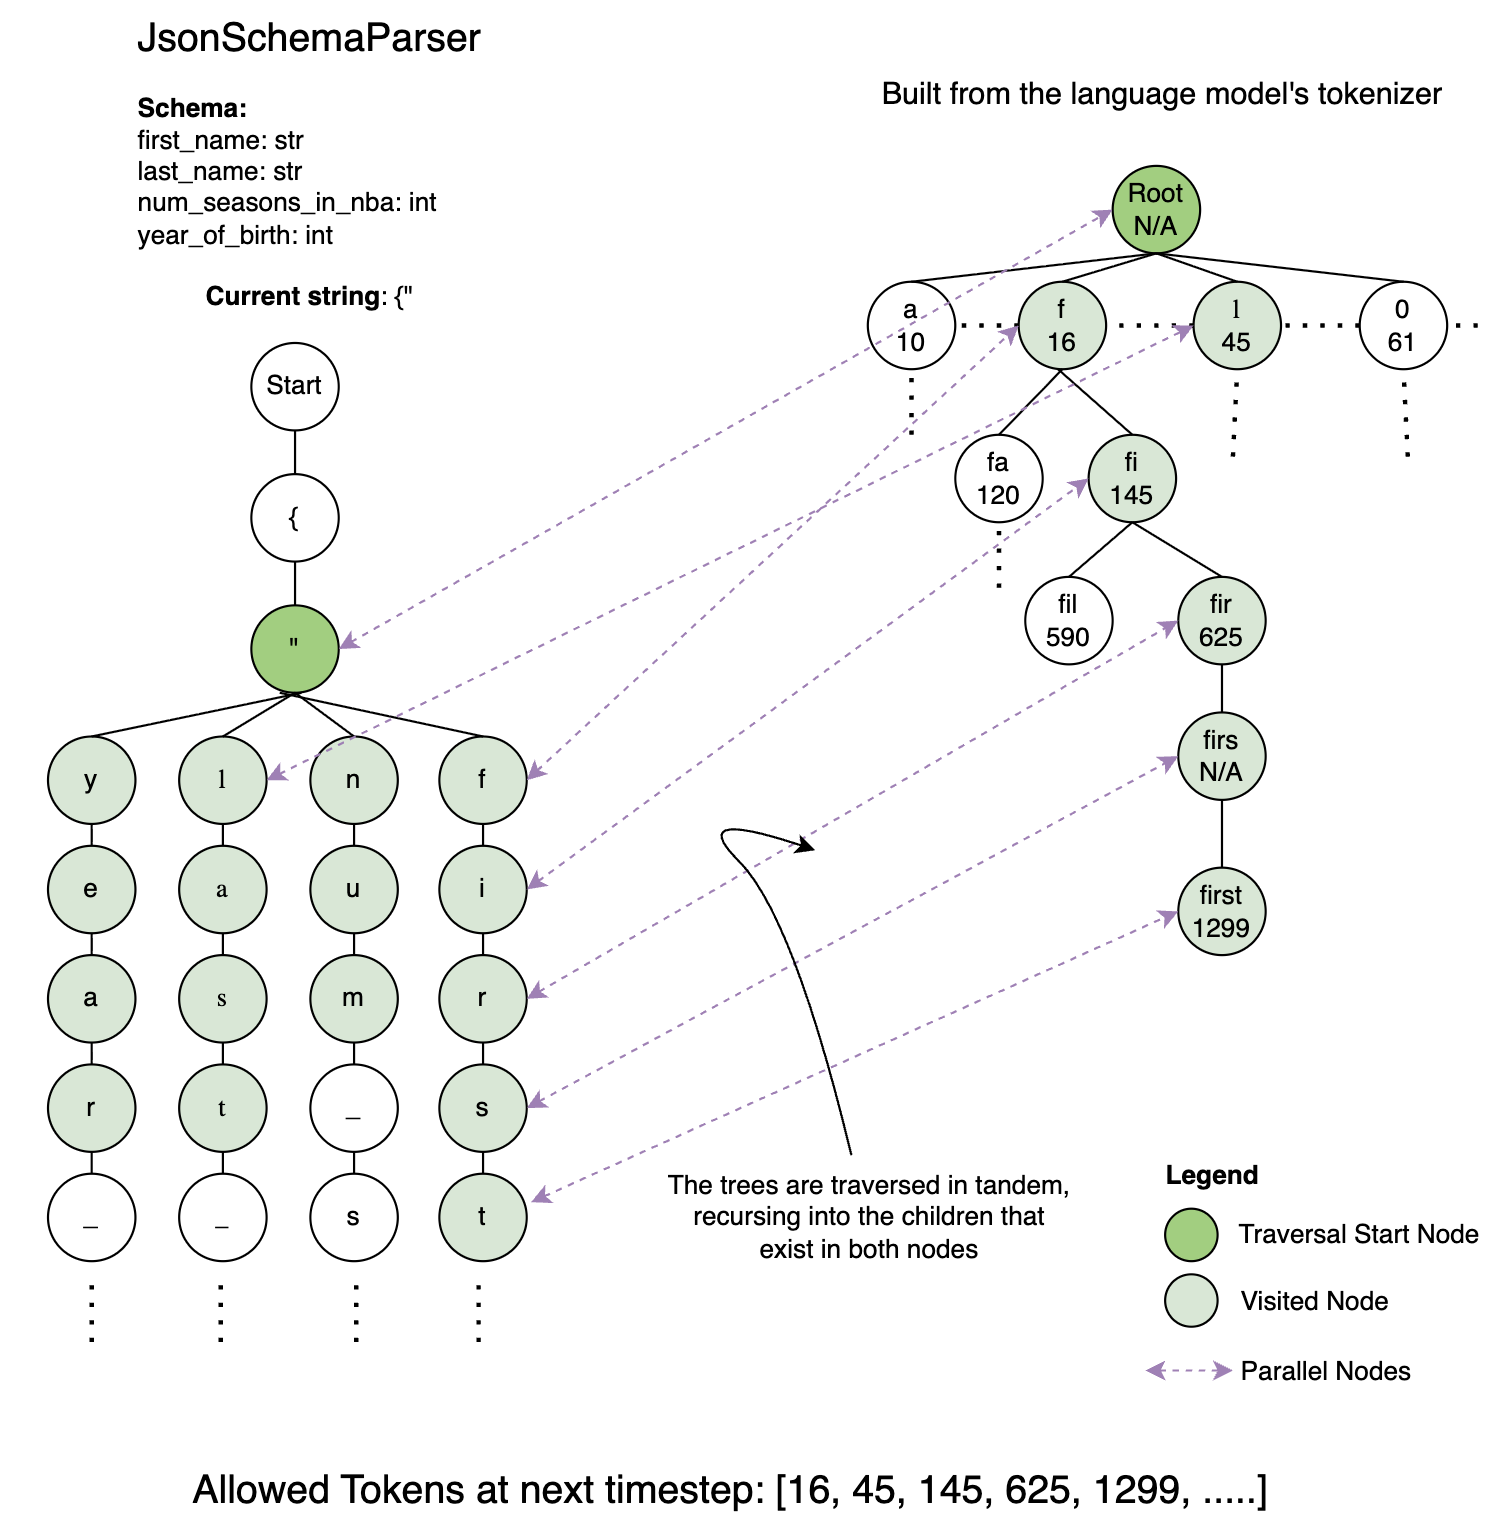
\includegraphics[width=0.7\textwidth]{Bilder/LMFormatEnforcer.png}
    \caption{LM Format Enforcer mechanism: intersecting a character-level parser with a tokenizer prefix tree to constrain structured generation by computing the set of allowed next tokens at each decoding step \cite{noamgat-no-date}.}
    \label{fig:lmfe_mechanism}
\end{figure}
\FloatBarrier

\section{Expert Agents}
\label{sec:Expert_agents}

This section describes the expert agents used in the basic multi-agent experiments. In this first stage of the pipeline, multiple experts assess the same claim in parallel and return structured outputs that can be aggregated into a single binary decision (aggregation strategies are described in the next section). The expert design is intentionally lightweight: experts are defined purely through prompting (role + constraints) and a shared output schema, enabling controlled comparisons across prompt variants and inference settings.

\subsection{Prompt-Based Experts}

The baseline prototype uses three prompt-defined expert agents: \textit{politics}, \textit{economy}, and \textit{health/science}. These three domains were selected because they represent the largest and most distinct topical clusters in the LIAR dataset 
(Section~\ref{sec:exploratory_domain_analysis}), covering the majority of training instances while remaining semantically separable enough to support meaningful domain specialization. All three experts use the same underlying backbone model, but differ in their system prompts, which specify (i) the domain perspective, (ii) the kinds of publicly verifiable evidence to prioritize, and (iii) a conservative decision policy that defaults to \texttt{False} when evidence is insufficient or ambiguous. Concretely:

\begin{itemize}
    \item \textbf{Politics expert.} Focuses on U.S.\ politics, elections, legislation, and public records, emphasizing verifiable sources such as roll calls, bill texts, statutes, and official filings.
    \item \textbf{Economy expert.} Focuses on macroeconomics, labor statistics, budgets, and taxation, emphasizing statistical agencies and budget institutions (e.g., BLS, BEA, CBO, Treasury/IRS) and requiring precise definitions of metrics and time ranges.
    \item \textbf{Health/science expert.} Focuses on healthcare policy, public health, and scientific evidence appraisal, emphasizing institutional sources (e.g., CDC, FDA, NIH, WHO) and peer-reviewed literature, and explicitly distinguishing correlation from causation when relevant.
\end{itemize}

Each expert receives the same claim (statement text) and produces a compact machine-readable JSON object with two fields: a binary verdict (\texttt{True} or \texttt{False}) and a short explanation (2--4 concise sentences). This shared interface is crucial for aggregation because it keeps the expert stage comparable across configurations while allowing domain-specific reasoning through the role prompts.

\paragraph{Subject conditioning}
To test whether topic metadata improves expert judgments, the expert prompts were evaluated both \emph{with} and \emph{without} injecting the LIAR subject string into the input.

\subsection{Fine-Tuned Experts}

For clarity, the experiments compare three expert implementations:
\begin{itemize}
    \item \textbf{Prompt-only backbones:} untuned models instructed via prompts.
    \item \textbf{Domain-general fine-tuning:} LoRA adapters trained on the full LIAR training set.
    \item \textbf{Domain-specific fine-tuning:} LoRA adapters trained on topical LIAR subsets (economy, politics, health/science).
\end{itemize}

Beyond prompt-only experts, two additional expert types use supervised adaptation via LoRA fine-tuning. In both cases, experts retain the same binary label space (\texttt{True}/\texttt{False}) but are trained to align more directly with the LIAR labeling function. For domain-specific fine-tuning, the training data is grouped into three coarse superlabels aligned with the expert roles: \textit{economy}, \textit{politics}, and \textit{health/science}. Separate adapters are trained per superlabel and evaluated on the full LIAR test set.

This design yields \emph{domain-specialized fine-tuned experts}: each expert is optimized on a subset of the training distribution that corresponds to its topical scope, while evaluation on the full LIAR test set provides a measure of cross-domain transfer and robustness. Fine-tuned experts are used in the multi-agent setting analogously to prompt-based experts: each produces an independent binary decision that can be combined by the aggregation mechanisms described in the next section.

\subsection{Domain-General vs.\ Domain-Specific Experts}

The prototype experiments contrast two forms of expertise:

\begin{itemize}
    \item \textbf{Domain-specific experts:} experts whose prompts (or fine-tuning data) target a particular topical area (politics, economy, health/science). The intended advantage is improved precision in the relevant domain, by encouraging the expert to rely on appropriate evidence standards and domain-relevant sources.
    \item \textbf{Domain-general experts:} experts that apply a generic fact-checking instruction without a strong topical constraint, relying on general world knowledge and broad instruction-following behavior. This form is less specialized but can be more robust when claims do not clearly belong to a single domain.
\end{itemize}

In the first multi-agent experiments, domain specificity is realized through prompt-defined roles applied to the untuned backbones. The fine-tuning experiments then introduce two supervised variants: domain-general fine-tuning on the full LIAR training set, and domain-specific fine-tuning on topical subsets aligned with the expert roles. The remainder of this chapter focuses on how expert outputs are aggregated into a single pipeline verdict; routing and additional control modules are introduced in the final framework chapter.

\section{Decision Mechanisms}

This section describes how the prototype multi-agent pipeline aggregates expert outputs into a single binary prediction.
Each expert returns a structured verdict (\texttt{True}/\texttt{False}) with a short justification.
Aggregation maps the set of expert outputs to one final label $\hat{y}$.
All aggregation strategies are evaluated under controlled conditions, keeping expert prompts and structured-output constraints fixed.

\subsection{Final Classification Strategy}
Let $K$ denote the number of experts. Each expert $i \in \{1,\dots,K\}$ produces a binary vote
$y_i \in \{\texttt{True},\texttt{False}\}$.
The pipeline computes the final prediction $\hat{y}$ using one of three aggregation mechanisms:
\begin{itemize}
    \item \textbf{Majority vote:} an unweighted rule where each expert contributes equally.
    \item \textbf{Router-weighted vote:} a weighted rule where a prompted router assigns claim-specific weights $w_i$.
    \item \textbf{Decision-agent aggregation:} a separate model that reads the expert outputs and generates the final verdict.
\end{itemize}

\subsection{Majority Vote}
With $K=3$ experts, majority vote selects the label supported by at least two experts:
\[
\hat{y} = \arg\max_{c \in \{\texttt{True},\texttt{False}\}} \sum_{i=1}^{3} \mathbb{1}[y_i = c].
\]
Because $K$ is odd, ties cannot occur in this setting.

\subsection{Router-Weighted Voting}
To test whether claim--domain alignment improves aggregation, a router assigns non-negative weights $w_i$ to experts on a per-claim basis. The final label is chosen by weighted voting:
\[
\hat{y} = \arg\max_{c \in \{\texttt{True},\texttt{False}\}} \sum_{i=1}^{K} w_i \cdot \mathbb{1}[y_i = c].
\]
Weights are normalized to sum to one, $\sum_{i=1}^{K} w_i = 1$, so that the scale of the vote is comparable across instances. In practice, higher weights are assigned to the expert whose domain is judged most relevant to the claim, while lower weights are assigned to less relevant experts.

\paragraph{Weight estimation.}
Router weights are produced by a separate routing model that predicts claim--domain relevance for the three expert domains (\texttt{politics}, \texttt{economy}, \texttt{health\_science}).
For each backbone family, the router uses the same underlying model as the experts in that configuration (i.e. \textsc{Gemma} routes \textsc{Gemma} experts, \textsc{Llama} routes \textsc{Llama} experts, and \textsc{DeepSeek} routes \textsc{DeepSeek} experts), so routing quality reflects the same base model capabilities as the downstream expert judgments.
The router receives the claim text and optionally the LIAR subject tags and is prompted to output a JSON object with three non-negative values in $[0,1]$.
To enforce a valid output format, generation is constrained using a JSON-schema-based decoder, ensuring that only the required keys are emitted.
The raw router outputs are post-processed by clipping each value to $[0,1]$ and renormalizing to sum to one.
If the router output cannot be parsed, a uniform fallback distribution $w_i=\tfrac{1}{3}$ is used.
The final weights are therefore comparable across instances and can be interpreted as a soft relevance distribution over experts.

\subsection{Decision-Agent Aggregation}
Decision-agent aggregation replaces rule-based voting with an additional adjudication step. A separate decision model receives the structured expert outputs (verdicts and short explanations) and produces the final verdict $\hat{y}$ (and an accompanying explanation). This mechanism can, in principle, discount weak or internally inconsistent expert justifications even when the raw votes are similar.

\paragraph{Structured outputs.} 
For all aggregation mechanisms, both expert responses and the final output are constrained to valid JSON via decoding-time enforcement (LM Format Enforcer), ensuring that intermediate outputs are reliably machine-readable and can be evaluated consistently.

\section{Multi-Agent Evaluation}

This section evaluates the two-stage multi-agent pipeline on the binary LIAR test set.
All systems use the same expert interface (binary verdict + short explanation) and differ only in (i) the expert implementation (prompt-only vs.\ fine-tuned), (ii) the aggregation mechanism, and (iii) whether LIAR subject tags are injected as additional metadata.

\subsection{Evaluation Metrics}

Performance is reported using standard binary classification metrics: accuracy, precision, recall, and $F_1$.
In addition, confusion matrices are provided to expose the underlying error structure (false positives vs.\ false negatives).
Following the binary reduction used throughout this thesis, $\texttt{True}$ is treated as the positive class when reporting precision, recall, and $F_1$.
For aggregation mechanisms (majority vote, weighted vote, decision-agent), metrics are computed on the full test set.

\subsection{Results}

Table~\ref{tab:multiagent_agg_subset} summarizes aggregation-only results for three model families (\textsc{Gemma}, \textsc{Llama}, \textsc{DeepSeek}) across three training regimes (basic model, LIAR-finetuned, domain-specific) and two input conditions (with vs.\ without LIAR subjects). Complete results for all models and configurations are reported in Appendix~E Table~\ref{tab:multiagent_all_results}.

\paragraph{Overall best configurations.}
The strongest results are backbone-dependent.
For \textsc{Gemma}, the best overall Macro-F1 is obtained with the decision-agent in the LIAR-finetuned regime without subjects (Acc $=0.631$, Macro-F1 $=0.604$), while majority voting achieves the highest accuracy in this regime (Acc $=0.644$, Macro-F1 $=0.595$); the gap reflects a more skewed prediction distribution under majority voting.
For \textsc{Llama}, router-weighted voting is consistently the strongest aggregation method, peaking in the LIAR-finetuned regime with subjects (Acc $=0.630$, Macro-F1 $=0.629$).
For \textsc{DeepSeek}, the largest improvement is achieved via domain-specific training combined with majority voting without subjects (Acc $=0.609$, Macro-F1 $=0.608$).

\paragraph{Aggregation mechanisms: decision-agent vs.\ voting.}
Across most settings, the decision-agent does not outperform the strongest voting rule in accuracy, though it sometimes yields a higher Macro-F1 by producing more balanced class predictions.
For \textsc{Gemma} in the LIAR-finetuned regime without subjects, majority voting achieves Acc $=0.644$ and Macro-F1 $=0.595$, while the decision-agent reaches Acc $=0.631$ and Macro-F1 $=0.604$; the higher Macro-F1 of the decision-agent reflects a less skewed prediction distribution despite lower accuracy.
A clearer advantage for voting holds for \textsc{Llama} in the LIAR-finetuned regime with subjects, where decision-agent aggregation (Acc $=0.603$, Macro-F1 $=0.599$) is below weighted voting on both metrics (Acc $=0.630$, Macro-F1 $=0.629$).
These comparisons suggest that rule-based aggregation is the more reliable default in this setting, while the decision-agent does not consistently exploit explanations to correct errors.

\paragraph{Majority vs.\ weighted voting depends on the backbone.}
Weighted voting behaves differently across model families.
For \textsc{Llama}, weighted voting consistently improves over majority voting in every listed training regime and subject condition, on both accuracy and Macro-F1.
For example, in the LIAR-finetuned regime without subjects, weighted voting increases performance from Acc $=0.597$, Macro-F1 $=0.585$ (majority) to Acc $=0.616$, Macro-F1 $=0.614$ (weighted).
With subjects, the gain remains visible (majority: Acc $=0.615$, Macro-F1 $=0.610$; weighted: Acc $=0.630$, Macro-F1 $=0.629$), indicating that routing weights correlate with useful expert selection for this backbone.
In contrast, \textsc{DeepSeek} often favors majority voting over weighted voting, particularly under domain-specific training (no subjects: majority Acc $=0.609$, Macro-F1 $=0.608$ vs.\ weighted Acc $=0.524$, Macro-F1 $=0.506$), suggesting that weighting can amplify failure modes when routing is miscalibrated.

\paragraph{Effect of training regime (basic vs.\ LIAR-finetuned vs.\ domain-specific).}
Training regime effects are strongest for \textsc{DeepSeek}.
In the LIAR-finetuned regime without subjects, majority voting reaches Acc $=0.531$ and Macro-F1 $=0.513$, while domain-specific training increases this to Acc $=0.609$ and Macro-F1 $=0.608$ indicating that role-aligned adaptation substantially stabilizes the expert ensemble for this backbone.
For \textsc{Gemma}, the LIAR-finetuned regime is clearly stronger than the basic model regime; for instance, under majority voting without subjects, performance rises from Acc $=0.549$, Macro-F1 $=0.535$ (basic model) to Acc $=0.644$, Macro-F1 $=0.595$ (LIAR-finetuned).
For \textsc{Llama}, the LIAR-finetuned regime also improves substantially over the basic model regime, but the overall outcome remains strongly controlled by the aggregation choice, with weighted voting consistently yielding the best results.

\begin{table}[t]
\centering
\scriptsize
\setlength{\tabcolsep}{3.5pt}
\renewcommand{\arraystretch}{1.05}
\caption{Aggregation-only results on \texttt{liar\_test} ($n = 1267$). Reported are Accuracy and Macro-F1 (unweighted average of $F_1$ over both classes) for three aggregation mechanisms: decision agent, majority vote, and weighted vote. Best Macro-F1 per row is highlighted in bold.}
\label{tab:multiagent_agg_subset}
\begin{adjustbox}{max width=\textwidth}
\begin{tabular}{@{}l p{2.8cm} c rr rr rr@{}}
\toprule
& & & \multicolumn{2}{c}{Decision Agent} & \multicolumn{2}{c}{Majority Vote} & \multicolumn{2}{c}{Weighted Vote} \\
\cmidrule(lr){4-5} \cmidrule(lr){6-7} \cmidrule(lr){8-9}
Train-Set & Model & Subj. & Acc & MF1 & Acc & MF1 & Acc & MF1 \\
\midrule
basic model     & gemma-7b-it           & no  & 0.551 & 0.539          & 0.549 & 0.535          & \textbf{0.563} & \textbf{0.554} \\
basic model     & gemma-7b-it           & yes & 0.566 & 0.562          & 0.571 & 0.566          & \textbf{0.576} & \textbf{0.572} \\
LIAR-finetuned  & gemma-7b-it           & no  & 0.631 & \textbf{0.604} & \textbf{0.644} & 0.595          & 0.643 & 0.597 \\
LIAR-finetuned  & gemma-7b-it           & yes & 0.627 & 0.610          & \textbf{0.636} & \textbf{0.612} & 0.630 & 0.607 \\
domain-specific & gemma-7b-it           & no  & 0.613 & 0.607          & 0.618 & 0.616          & \textbf{0.631} & 0.605 \\
domain-specific & gemma-7b-it           & yes & 0.631 & 0.624          & \textbf{0.638} & \textbf{0.628} & 0.633 & 0.625 \\
\midrule
basic model     & Llama-3.1-8B-Instruct & no  & 0.474 & 0.413          & 0.470 & 0.392          & \textbf{0.477} & \textbf{0.424} \\
basic model     & Llama-3.1-8B-Instruct & yes & \textbf{0.479} & \textbf{0.427} & 0.473 & 0.399        & 0.474 & 0.421 \\
LIAR-finetuned  & Llama-3.1-8B-Instruct & no  & 0.583 & 0.573          & 0.597 & 0.585          & \textbf{0.616} & \textbf{0.614} \\
LIAR-finetuned  & Llama-3.1-8B-Instruct & yes & 0.603 & 0.599          & 0.615 & 0.610          & \textbf{0.630} & \textbf{0.629} \\
domain-specific & Llama-3.1-8B-Instruct & no  & 0.543 & 0.515          & 0.524 & 0.482          & \textbf{0.565} & \textbf{0.550} \\
domain-specific & Llama-3.1-8B-Instruct & yes & 0.543 & 0.523          & 0.533 & 0.498          & \textbf{0.567} & \textbf{0.555} \\
\midrule
basic model     & deepseek-llm-7b-base  & no  & 0.491 & 0.451          & \textbf{0.496} & \textbf{0.460} & 0.492 & 0.453 \\
basic model     & deepseek-llm-7b-base  & yes & \textbf{0.516} & \textbf{0.500} & 0.507 & 0.488        & 0.514 & 0.493 \\
LIAR-finetuned  & deepseek-llm-7b-base  & no  & 0.502 & 0.470          & \textbf{0.531} & \textbf{0.513} & 0.484 & 0.437 \\
LIAR-finetuned  & deepseek-llm-7b-base  & yes & \textbf{0.525} & \textbf{0.514} & 0.522 & 0.510        & 0.489 & 0.450 \\
domain-specific & deepseek-llm-7b-base  & no  & 0.527 & 0.516          & \textbf{0.609} & \textbf{0.608} & 0.524 & 0.506 \\
domain-specific & deepseek-llm-7b-base  & yes & \textbf{0.519} & \textbf{0.509} & 0.526 & 0.512        & 0.491 & 0.450 \\
\bottomrule
\end{tabular}
\end{adjustbox}
\end{table}

\subsection{Ablation Studies}

Ablations isolate three factors: (i) subject conditioning, (ii) aggregation strategy, and (iii) training regime.

\paragraph{Subject conditioning (with vs.\ without subjects).}
Subject tags show small and inconsistent effects.
For \textsc{Gemma} in the LIAR-finetuned regime, subject injection slightly reduces Macro-F1 under majority voting (from $0.595$ to $0.612$) and weighted voting (from $0.597$ to $0.607$), while the decision-agent improves marginally (from $0.604$ to $0.610$).
For \textsc{Llama}, subject tags tend to help in the strongest configurations: in the LIAR-finetuned regime under weighted voting, Macro-F1 improves from $0.614$ (no subjects) to $0.629$ (with subjects).
For \textsc{DeepSeek}, the effect varies by training regime; in the domain-specific regime, adding subjects reduces majority vote Macro-F1 from $0.608$ (no subjects) to $0.512$ (with subjects), a substantial drop indicating that subject metadata interacts poorly with domain-specific adaptation for this backbone.
Overall, subject metadata behaves as an auxiliary cue that can help under some routing conditions but is not robustly beneficial.

\paragraph{Aggregation ablation: majority vs.\ weighted vs.\ decision-agent.}
Majority vote provides a stable baseline, while weighted voting is beneficial mainly when routing is reliable.
For \textsc{Llama}, weighted voting consistently improves Macro-F1 over majority voting across all regimes and subject settings.
For \textsc{DeepSeek}, majority voting is often preferable in terms of both accuracy and Macro-F1, particularly under domain-specific training where weighted voting underperforms sharply.
Across backbones, decision-agent aggregation is rarely the strongest option: it achieves the best Macro-F1 only for \textsc{Gemma} in the LIAR-finetuned no-subjects regime ($0.604$ vs.\ $0.595$ for majority voting), where its more balanced class predictions yield a small advantage despite lower accuracy.

\paragraph{Training regime ablation: basic vs.\ LIAR-finetuned vs.\ domain-specific.}
Domain-specific training yields the strongest gains for \textsc{DeepSeek}, especially when paired with majority voting without subjects ($\Delta$Macro-F1 $= +0.095$ over LIAR-finetuned majority vote).
For \textsc{Gemma} and \textsc{Llama}, the LIAR-finetuned regime is substantially stronger than the basic model regime, while domain-specific variants remain competitive but do not uniformly surpass the best LIAR-finetuned configurations on Macro-F1.

\paragraph{Summary.}
Taken together, the results indicate that (i) simple voting rules are strong and reliable aggregators, (ii) the usefulness of router-weighted voting is backbone-dependent---consistently beneficial for \textsc{Llama} but counterproductive for \textsc{DeepSeek} under miscalibrated routing---and (iii) domain-specific training is particularly important for stabilizing weaker backbones, as evidenced by the large Macro-F1 gains for \textsc{DeepSeek}. The Macro-F1 metric proves especially informative here: several configurations that appear similar in accuracy differ meaningfully in class balance, with majority voting tending to produce more skewed predictions than the decision-agent in high-recall regimes.

\paragraph{Limitations and motivation for the final framework.}
Despite these improvements over single-model baselines, the prototype reveals three key limitations that motivate the extended framework in Chapter~\ref{chap:final_framework}. First, all claims are evaluated by all three experts regardless of their actual domain, which is inefficient and introduces noise from irrelevant expert perspectives. Second, the three-domain taxonomy is coarse and may not capture the full topical diversity of LIAR. Third, the pipeline has no mechanism to filter non-verifiable or underspecified claims, which forces experts into speculative decisions. These limitations are addressed in the final framework through domain routing, finer-grained taxonomies, and a checkability gate.